\chapter{Experimente}
\label{ch:experiment}
Trotz der vielen unterschiedlichen Techniken und Methoden aus dem letzten Kapitel, sind die Modelselektion und die Wahl der richtigen Methoden weiterhin sehr problemspezifisch.

Um für ein Lernproblem ein passendes Model zu finden, beschreiben \cite{Bengio2007b} drei essentielle Komponenten, die mit entsprechendem Vorwissen spezifiziert werden müssen:
\begin{enumerate}
\item Die Repräsentation und Vorverarbeitung der Daten

\item Die Architektur der Maschine oder des Neuronalen Netzes

\item Die Optimierung der Fehlerfunkion sowie Regularisierung
\end{enumerate}

Dieses Kapitel gliedert diese drei Komponenten in die Bereiche Modelselektion, Training und Visualisierung. Als Datenmaterial (vgl. Abbildung \ref{fig:6_samples}) dienen die beiden folgenden bekannten Datensätze:

\begin{itemize}
\item MNIST\footnote{MNIST-Datensatz: \url{http://yann.lecun.com/exdb/mnist/} (10.09.2015)} \textemdash\space Der MNIST-Datensatz handgeschriebener Ziffern besteht aus 60000 Trainingsbeispielen und 10000 Testbildern. Es stellt eine Untermenge des größeren NIST-Datensatzes dar. Die binarisierten Bilder sind $28 \times 28$ Pixel groß und die Ziffern zentriert. Richtwerte für Fehlerraten liegen mit \textit{Data Augmentation} bei 0.23 \% (\cite{Ciresan2012}), mit Vortraining bei 0.53 \% (\cite{Jarrett2009}) und ohne Vorverarbeitung bei 0.7 \% (\cite{Ranzato2006}). Das beste Ergebnis erreicht das \textit{DropConnect Network} von \cite{Zeiler2013} mit 0.21 \% Fehler ohne \textit{Data Augmentation}.

\item CIFAR-10\footnote{CIFAR-10-Datensatz: \url{http://www.cs.toronto.edu/~kriz/cifar.html} (10.09.2015)} \textemdash\space Der CIFAR-10-Datensatz besteht aus 50000 $32 \times 32 $ Pixel großen Trainingsbeispielen und 10000 Testbildern. Die Bilder sind aufgeteilt in 10 Klassen: Flugzeug, Auto, Vogel, Katze, Rotwild, Hund, Frosch, Pferd, Schiff und Lastwagen. Richtwerte für Fehlerraten liegen mit \textit{Data Augmentation} bei 9.3 \% (\cite{Zeiler2013}), ohne bei 11.7 \% (\cite{Goodfellow_maxout_2013}). Mit unüberwachten Vortraining erreichen \cite{Masci2011} 21.8 \%, ohne 22.5 \% Fehler.  Mit dem Standard Cuda-Convnet werden ohne \textit{Data Augmentation} und Vorverarbeitung ein Fehler von 18 \% erreicht\footnote{Cuda-Convnet Projekt: \url{https://code.google.com/p/cuda-convnet/} (10.09.2015)}. Das beste Ergebnis mit 8.2 \% Fehler erzielt das \textit{Deeply-Supervised Net} von \cite{Lee2014} mittels \textit{Data Augmentation}.
\end{itemize}

\begin{figure}
\centering
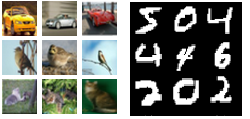
\includegraphics[width=0.5\linewidth]{images/6_samples}
\caption[]{CIFAR-10 Beispiele (links) und MNIST-Beispiele (rechts)}
\label{fig:6_samples}
\end{figure}


\section{Modelselektion}
Typischerweise bestehen die zur Verfügung stehenden Daten aus Trainingsdaten und Testdaten.
Um die verschiedenen Ergebnisse zu vergleichen, werden von den vorhandenen Trainingsdaten zufällige Beispiele entnommen. Wie Abbildung \ref{fig:6_validationset} zeigt, bilden diese Daten die Validierungsdaten, welche zur Überwachung des Trainings und zur Bestimmung der aktuellen Performanz verwendet werden. Die Testdaten werden verwendet, um das Model mit anderen Modellen zu vergleichen und dürfen nicht in die Validierung einbezogen werden \cite[vgl. z. B.][S. 222]{Hastie2009}. Eine Erweiterung zu diesem Verfahren ist die Kreuzvalidierung, wobei die Trainingsdaten in $k$ Blöcke unterteilt werden und das Training mehrfach mit unterschiedlichem Block zur Validierung durchgeführt wird. Die Performanz des Modells ergibt sich aus dem Durchschnitt der einzelnen Trainings \cite[vgl. z. B.][Kap. 7.2, S. 219]{Bengio2015}.  

\begin{figure}[H]
\centering

\includegraphics[width=0.6\linewidth]{images/6_validationset}
\caption[]{Aufteilung der Trainingsdaten in Trainings- und Validierungsdaten}
\label{fig:6_validationset}
\end{figure}

\subsection{Modelarchitektur}
Anfang der 2000er war es gängige Praxis die Anzahl der Parameter entsprechend der Menge an Trainingsdaten zu wählen
\cite[vgl.][S. 95 f.]{Zander2001}. 
Dies ist beispielsweise auch am bekannten \textit{LeNet 5} von \cite{LeCun1998} mit 60.000 freien Parametern für das Training des MNIST-Datensatzes zu erkennen.
Neuere vorgestellte Architekturen beinhalten deutlich mehr freie Parameter \cite[vgl. z. B.][]{Andrade2014}. Aufgrund besserer Techniken zur Regularisierung, wie beispielsweise Dropout, ist es möglich eine bedeutend größere Zahl an Gewichten als Trainingsdaten zu verwenden, ohne dabei mit \textit{Overfitting} konfrontiert zu werden \cite[vgl.][]{Bengio2012}.
Aufgrund empirischer Untersuchungen hat sich herausgestellt, dass die frühere angewandte Pyramidenform für die Layer-Größen (z. B. \textit{LeNet 5}: 6-16-120/84-10)\footnote{Die Darstellung der Modellarchitektur in der Form 6-16-120/84-10 steht für drei Convolution-Layer mit 6, 16, 120 \textit{Feature-Maps} und einem Hidden-Layer mit 84 sowie einem Output-Layer mit 10 Neuronen. Zur Klassifikation wird stets die Softmax-Regression angewandt.} suboptimal ist und gleichbleibende Größen der Schichten zu bevorzugen sind \cite[vgl.][]{Larochell2009}. 

Dieser Teil stellt die für die Experimente herangezogenen Architekturen der Modelle vor. In allen Experimenten werden, aufgrund ihrer guter Ergebnisse, die ReLu-Funktionen als Aktivierung und Max-Pooling als Pooling-Methode verwendet (vgl. z. B. \cite{Krizhevsky2012} und \cite{Simonyan2014}). Außerdem wird standardmäßig kein Padding angewandt. Dies bedeutet, dass die Größe nach einem Convolution-Layer mit Filtergröße $K \times K$ auf $N - K + 1 \times N - K + 1$ schrumpft.\\

\textit{LeNet 5+}\\
Die erste vorgestellte Architektur ist ein erweitertes \textit{LeNet 5} und orientiert sich an dem von \cite{Ranzato2006} vorgestellten Modell. 
Es wird mit 50-50/200-10 abgekürzt und umfasst im Detail die folgenden sechs Schichten:
\begin{enumerate}
\setlength{\itemsep}{0pt}
\item Convolution-Layer: 50 \textit{Feature-Maps} mit $5 \times 5$ Filtermasken
\item Pooling-Layer:	$2 \times 2$ Filtermasken
\item Convolution-Layer: 50 \textit{Feature-Maps} mit $5 \times 5$ Filtermasken
\item Pooling-Layer:	$2 \times 2$ Filtermasken
\item Hidden-Layer: 200 Neuronen
\item Output-Layer: 10 Neuronen mit Cross-Entropy Fehlermaß
\end{enumerate}
Dieses Netz wird für das Training der MNIST-Daten verwendet und umfasst für die Eingabe der Größe $28 \times 28 \times 1$ 63.750 Gewichte in den Convolution-Layern und 162.000 Gewichte im MLP. Insgesamt enthält es somit 223.950 Gewichte. \\

\textit{Net-7} \\
Das zweite vorgestellte Architektur besitzt eine zusätzliche Schicht und besteht folglich aus sieben Schichten. Es orientiert sich an den Modellen von \cite{Hinton2012} und \cite{Zeiler2013b}.
Das Modell wird mit 64-64-64/64-10 abgekürzt und umfasst im Detail die folgenden sieben Schichten:
\begin{enumerate}
\setlength{\itemsep}{0pt}
\item Convolution-Layer: 64 \textit{Feature-Maps} mit $5 \times 5$ Filtermasken
\item Pooling-Layer:	$2 \times 2$ Filtermasken
\item Convolution-Layer: 64 \textit{Feature-Maps} mit $5 \times 5$ Filtermasken
\item Pooling-Layer:	$2 \times 2$ Filtermasken
\item Convolution-Layer: 64 \textit{Feature-Maps} mit $5 \times 5$ Filtermasken
\item Hidden-Layer: 64 Neuronen
\item Output-Layer: 10 Neuronen mit Cross-Entropy Fehlermaß
\end{enumerate}
Dieses Netz wird für die CIFAR-10-Daten verwendet. Aufgrund der größeren Eingabe von $32 \times 32$ ist es möglich, drei Convolution-Layer zu verwenden, da nach zwei Convolution- und Pooling-Layern noch die Eingangsgröße von $5 \times 5$ für den dritten Convolution-Layer verbleibt. Dieses Netz umfasst für die Eingabe der Größe $32 \times 32 \times 3$ 209.600 Gewichte in den Convolution-Layern und 10.496 Gewichte im MLP.  Insgesamt enthält es somit 220.096 Gewichte. \\
%Parameters: 3*25*64 = 4800		32 - 4 = 28 / 2 = 14
%			64*64*25 = 102400	14 - 4 = 10 / 2 = 5 %
%			64*64*25 = 102400
%			64*64		= 4096
%			64*10			6400
%		=> 220 096

In diesem Zusammenhang ist die Analyse von \cite{Zeiler2014} von Bedeutung. Hier wird festgestellt, dass zum einen die Gesamttiefe des Netzes wichtig ist und zum anderen die Größe der Hidden-Layer keinen großen Einfluss auf die Performanz hat. Darüber hinaus hat die Größe der mittleren Convolution-Layer enormen Einfluss auf das Ergebnis, während ein zu großer Hidden-Layer nach den Convolution-Layern ohne Regularisierung zu \textit{Overfitting} führt.

%\subsubsection{Speicherbedarf}
%Da es allerdings nicht praktikabel ist, unnötige Rechenressourcen zu belegen, lohnt es sich dennoch das Modell möglichst klein zu halten. 	
%An dieser Stelle soll deshalb exemplarisch für den MNIST-Datensatz der für das \textit{LeNet 5+} benötigte Speicherplatz berechnet werden.
%Grundsätzlich ist der Speicherbedarf in zwei Kategorien einzuteilen: Aktivierungen und Gewichte und Schwellwerte.
%Für die Aktivierungen müssen nach den ersten Schicht $24*24*50=28.800$, nach der dritten Schicht $8*8*50=3.200$ und nach der fünften Schicht $200$ Aktivierungen gespeichert werden. Das macht inklusive der Eingabe bei doppelter Genauigkeit $257.944$ Bytes pro Trainingsbeispiel.
%Für die Gewichte und Schwellwerte sind entsprechend $(223.950 + 310)*8 = 1.794.080$ Bytes zu reservieren. Hinzukommt ein Faktor 4 für Gradient, Momentum und Hesse-Approximation. Insgesamt benötigt das Modell folglich 7.176.320 Bytes für die Parameter. Bei Parallelisierung multipliziert sich der benötigte Speicher entsprechend mit den Threads, wobei lediglich der Speicher für den Gradient extra berechnet werden muss.
%Die wichtigste Stellgröße für den Speicherbedarf ist somit die Wahl der Größe eines \textit{Mini-Batch}, da dieser unmittelbare Auswirkung auf den benötigten Speicher hat.


\subsection{Vorverarbeitung}
Die beiden verwendeten Datensätze werden auf verschiedene Arten vorverarbeitet. Somit werden mehrere Versionen erzeugt. Zunächst wird der Wertebereich beider Datensätze auf Werte zwischen 0 und 1 skaliert. Der MNIST-Datensatz wird im Anschluss lediglich zentriert, indem der Mittelwert pro Pixel subtrahiert wird. Der ebenfalls zentrierte CIFAR-10-Datensatz wird als CIFAR-10A bezeichnet. Eine zweite Variante, CIFAR-10B genannt, wird in den HSV-Farbraum\footnote{Der HSV-Farbraum bietet den Vorteil, dass die Farbe lediglich im H-Kanal codiert ist und die Kanäle S und V Informationen über Sättigung und Helligkeit enthalten.} transformiert und ebenfalls zentriert. 
\textit{Data-Augmentation} kann die Performanz immens verbessern. Hierauf wird allerdings im Folgenden verzichtet, da nicht die absolute Leistung des Modells von Interesse ist, sondern Unterschiede der einzelnen Aspekte und Methoden vorgestellt werden. 

Da im Rahmen der Experimente oftmals \textit{Early Stopping} zum Einsatz kommt, wird die Zentrierung der Daten lediglich mit den echten Trainingsdaten und nicht mit den Validierungsdaten berechnet. Im Anschluss werden die Validierungs- und Testdaten entsprechend transformiert. 


\section{Trainingsmethode}
Dieses Kapitel beschreibt die verschiedenen Experimente im Bereich des Trainings. Diese betreffen die Bereiche unüberwachtes Vortraining, Initialisierung, Gradientenabstieg und Regularisierung.

Als Größe für einen \textit{Mini-Batch} wird in Anlehnung an \cite{Bengio2012} immer eine Größe von 40 gewählt. Dies ermöglicht, dass bei 20 Threads jeweils zwei Trainingsbeispiele pro Thread parallel gerechnet werden können.
Zur Begrenzung der Trainingszeit sowie zur Vermeidung von \textit{Overfitting} kommt die Methode \textit{Early-Stopping} zum Einsatz. Wie zu Beginn des Kapitels beschrieben, müssen die Trainingsdaten dazu jeweils in ein Trainings- und Validierungsset unterteilt werden. Das Validierungsset umfasst stets 10 \% der Trainingsbeispiele und das Trainingsset somit entsprechend $55.000$ bei MNIST beziehungsweise $45.500$ bei CIFAR-10. \textit{Early-Stopping} wird derart verwendet, sodass das Modell immer fünf Durchläufe über das Trainingsset (Epochen) auf eine Verbesserung des Validierungsfehler wartet und das Training ansonsten abbricht. Im Anschluss gibt es verschiedene Varianten mit den verbliebenen Validierungsdaten umzugehen. \cite{Goodfellow_maxout_2013} beschreiben hierfür zwei Strategien: Bei Nutzung der ersten Strategie werden die Daten zur Trainingsmenge hinzugefügt und solange weiter trainiert bis der Validierungsfehler dem des Trainings entspricht. Wird die zweite Strategie verwendet, so wird das gesamte Training neu gestartet und solange trainiert bis der Trainingsfehler dem des Fehlers aus dem \textit{Early-Stopping}-Lauf entspricht. 

Im Rahmen dieser Arbeit wird allerdings die etwas praktikablere Methode von \cite{Ranzato2006} angewandt. Die Validierungsdaten werden hierbei ebenso am Ende des Trainings mit den Trainingsdaten kombiniert, jedoch wird maximal weitere 5 Epochen mit der gesamten Trainingsmenge trainiert. Das Training wird früher abgebrochen, falls sich der Validierungsfehler nicht weiter verbessert. Anschließend wird der Fehler auf den Testdaten berechnet, um die Ergebnisse der einzelnen Experimente zu vergleichen. 


\subsection{Vortraining}
\label{ch:pretrain} 
In diesem Teil soll das unüberwachte Vortraining untersucht werden. Dessen Ziel ist es, die erste Schicht im Modell zu initialisieren (vgl. z. B. \cite{Ranzato2006} und \cite{Masci2011}). Dabei sollen die enthaltenen Gewichte mittels des in Kapitel \ref{ch:autoenc} beschriebenen Convolutional Autoencoder trainiert werden. Alle Gewichte werden mittels der Standard-Initialisierung initialisiert (vgl. Kapitel \ref{ch:6_init}). Die Lernrate muss mit $\eta = 1^{-4}$ sehr klein gewählt werden, da das Modell im Rahmen dieser Experimente ansonsten divergiert. 

\subsubsection{MNIST}
Im ersten Experiment wird kein Input-Dropout, beziehungsweise keine Maskierung vorgenommen. Als Pooling-Methode kommt das Max-Pooling zum Einsatz. Die Trainingsdaten liefert der MNIST-Datensatz mit 55.000 Trainings- und 5.000 Validierungsbeispielen.
Bei Standard-Initialisierung und SGD mit einer Lernrate von $\eta = 1^{-4}$ erreicht das Model nach 39 Epochen ein Minimum mit einem MSE von $0.31$ auf den Testdaten.

Abbildung \ref{fig:6_mnist_autoencoder_combined} zeigt gelernte $5 \times 5$ Filtermasken der ersten Schicht auf der linken Seite.
\begin{figure}[H]
\centering
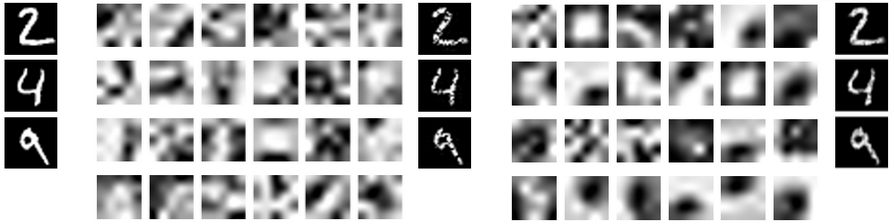
\includegraphics[width=0.9\linewidth]{images/6_mnist_autoencoder_combined}
\caption[]{Mit dem Convolutional Autoencoder trainierte Filtermasken und Rekonstruktionen der ersten \textit{LeNet 5+}-Schicht auf Basis des MNIST-Datensatz. Max-Pooling (links) und Max-Pooling und Maskierung (rechts)}
\label{fig:6_mnist_autoencoder_combined}
\end{figure}

Das zweite Experiment verwendet dieselbe Konfiguration, allerdings wird nun zusätzlich ein Input-Dropout von 30 \% verwendet.
Nach 14 Epochen erreicht das Modell einen MSE von $2.07$ auf den Testdaten. Abbildung \ref{fig:6_mnist_autoencoder_combined} zeigt die gelernten $5 \times 5$ Filtermasken der ersten Schicht auf der rechten Seite.
Die Filter des \textit{Denoising Autoencoder} aus dem zweiten Experiment wirken robuster und die Rekonstruktionen glatter. Deshalb werden diese für weitere Experimente beibehalten.

\subsubsection{CIFAR-10}
Im ersten Experiment wird kein Input-Dropout, beziehungsweise keine Maskierung vorgenommen. Als Pooling-Methode kommt ebenfalls das Max-Pooling zum Einsatz. Die Trainingsdaten stellt der CIFAR-10A/B-Datensatz mit 45.500 Trainings- und 4.500 Validierungsbeispielen.
Bei Standard-Initia\-lisierung und SGD mit einer Lernrate von $\eta = 1^{-4}$ erreicht das Modell auf den Testdaten (CIFAR-10A) nach 30 Epochen einen MSE von $74.06$ ohne Maskierung und $80.1$ mit Maskierung. Mit CIFAR-10B und Maskierung erreicht das Modell nach 20 Epochen einen deutlich besseren MSE von $26.2$ auf den Testdaten. 
Abbildung \ref{fig:6_cifar_autoencoder_combined_2} zeigt eine Auswahl der $5 \times 5$ Filtermasken der ersten Schicht in Graustufen. Es ist deutlich zu sehen, dass die Filter des CIFAR-10A optisch robuster wirken, während die Filter des CIFAR-10B sehr verrauscht sind.

\begin{figure}[H]
\centering
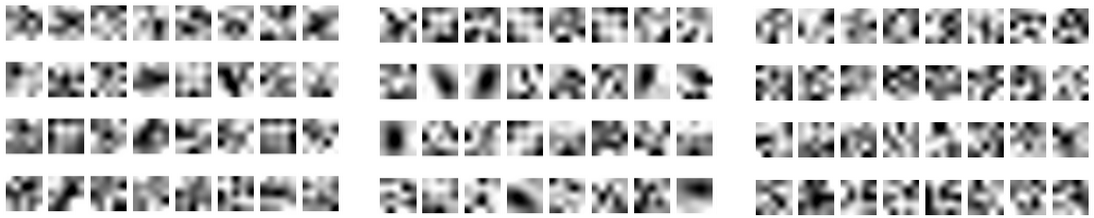
\includegraphics[width=1.0\linewidth]{images/6_cifar_autoencoder_combined_2}
\caption[]{Mit dem Convolutional Autoencoder trainierte Filtermasken der ersten \textit{Net-7}-Schicht auf Basis des CIFAR-10-Datensatz. CIFAR-10A: Max-Pooling (links), Max-Pooling und Maskierung (mitte) CIFAR-10B: Max-Pooling und Maskierung (rechts)}
\label{fig:6_cifar_autoencoder_combined_2}
\end{figure}

Für die weiteren Experimente werden jeweils die Filter aus dem Training mit Maskierung beibehalten.

\subsection{Initialisierung}
\label{ch:6_init}
In diesem Abschnitt werden verschiedene Initialisierungsmethoden verglichen. Als Basis dient in allen Beispielen der standardmäßige SGD mit einer \textit{Mini-Batch}-Größe von 40. Als Lernrate wird der universelle Wert $\eta = 0.01$ gewählt und es werden wieder 10 \% der Trainingsdaten zur Validierung verwendet. Tabelle \ref{tab:6_initialisierung} zeigt die jeweils erreichten Fehlerraten nach einer Epoche Training.

\begin{table}[H]

\centering
\begin{tabular}{c|c|c|c}
 	 			&   Standard		&  Xavier  	 	&  Vortraining 	 	\\ 
 	 			&     (mit $\sigma = 0.1$)		&  $~$  	 	&   (mit $\sigma = 0.1$)	 	\\ 
\hline MNIST 	&  	16.2/16.2 \%	&  	1.9/6.0   \% &  12.1/12.2 \%									\\
\hline CIFAR-10A&  	88.0/89.8 \%   &  	55.0/63.0 \% &  87.2/89.8 \%  				\\  
				&  	(68.4/72.2 \%)  &  	$~$ 		 &  (67.2/71.6 \%) 				\\  
\hline CIFAR-10B&  	88.0/89.8 \%	&  	54.6/62.2 \% &  87.2/89.8 \%		\\  
				&  	(66.8/71.4 \%)  &  	$~$ 		 &  (64.8/68.0 \%) 				\\  
\end{tabular} 
\caption{Fehler auf den Trainings-/Validierungsdaten nach einer Epoche (Ep.) Training}
\label{tab:6_initialisierung}
\end{table}

\subsubsection{Standard-Initialisierung}
Bei der Standard-Initialisierung werden alle Gewichte mit $W \sim \mathcal{N} (0,0.01)$ ini\-tialisiert. Abbildung \ref{fig:6_xavier_initialization} (mitte) zeigt pro Schicht die Verteilung der Werte im Gradienten über die erste Epoche beim Training des MNIST-Datensatz. Es fällt auf, dass die Varianzen über die verschiedenen Schichten gleich groß sind und somit kein \textit{Vanishing-Gradient}-Effekt erkennbar ist. Auch die angegebenen Fehlerraten in Tabelle \ref{tab:6_initialisierung} zeigen einen deutlichen Trainingsfortschritt.

\begin{figure}[H]
\centering
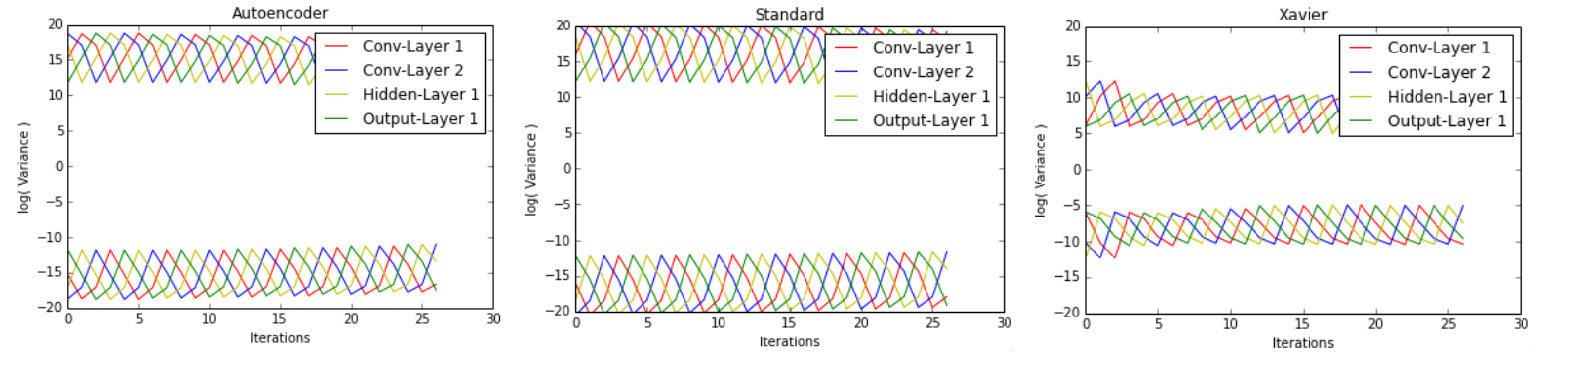
\includegraphics[width=1.0\linewidth]{images/6_xavier_initialization}
\caption[]{Log-Varianzen des Gradienten (gespiegelt) der einzelnen Schichten während der ersten Epoche des Trainings auf dem MNIST-Datensatz.}
\label{fig:6_xavier_initialization}
\end{figure}

Betrachtet man das Training mit CIFAR-10A/B in Abbildung \ref{fig:6_xavier_initialization_cifar}, zeigen die Varianzen der Werte im Gradienten ein ähnliches Bild wie beim MNIST. Allerdings sind die Varianzen hier kleiner (siehe Log-Varianz). Außerdem findet während der ersten Epoche kein erkennbarer Trainingsfortschritt statt. Dies deutet darauf hin, dass die Standard-Initialisierung nicht optimal für dieses Problem ist. Werden stattdessen die Gewichte mit $W \sim \mathcal{N} (0,0.1)$ initialisiert, sind die Varianzen größer und das Netz trainiert, was sich in den Werten in Tabelle \ref{tab:6_initialisierung} zeigt.


\subsubsection{Xavier-Initialisierung}
Bei der Xavier-Initialisierung werden alle Gewichte in Schichten mit ReLu-Aktivierungsfunktionen mittels $W \sim \mathcal{N} (0,\sqrt{2/fan_{out}})$ initialisiert. Die Abbildungen \ref{fig:6_xavier_initialization} und \ref{fig:6_xavier_initialization_cifar} (rechts) zeigt die Verteilung der Werte im Gradienten während der ersten Epoche pro Schicht. Im Vergleich zu den anderen Ini\-tialisierungstechniken sind die Varianzen insgesamt deutlich größer und das Modell erreicht bereits nach der ersten Epoche mit 6.0 \% (MNIST) respektive 63.0 und 64.2 \% (CIFAR-10A/B) sehr gute Fehlerraten auf den Validierungsdaten.

\subsubsection{Initialisierung durch Vortraining}
Nun werden die Gewichte mittels den gelernten Filtern aus Kapitel \ref{ch:pretrain} initialisiert. 
Die Abbildungen \ref{fig:6_xavier_initialization} und \ref{fig:6_xavier_initialization_cifar} (links) zeigen die Verteilung der Werte im Gradienten über die ersten Epoche pro Schicht. Beim MNIST-Datensatz ist zu erkennen, dass die Varianzen insgesamt zwar kleiner sind als bei der Xavier-Initialisierung, allerdings im Vergleich zur Standard-Initialisierung gegen Ende der Epoche größer werden. In der Folge führt diese Initialisierung zu einem besseren Ergebnis als bei Verwendung der Standard-Initialisierung, was Tabelle \ref{tab:6_initialisierung} zeigt. 
Anders verhält es sich beim CIFAR-Datensatz. Sowohl bei Verwendung der Datensätze CIFAR-10A/B als auch der Standard-Initialisierung findet in der ersten Epoche kein erkennbares Training statt und die Varianzen sind sehr klein. Analog zur Standard-Initialisierung findet ein Trainingsfortschritt statt, sobald die Standardabweichung im restlichen Netz auf $\sigma = 0.1$ erhöht wird. In diesem Modus erreicht das Netz binnen einer Epoche einen etwas geringeren Fehler als die gesamtheitliche Standard-Initialisierung.


\begin{figure}[H]
\centering
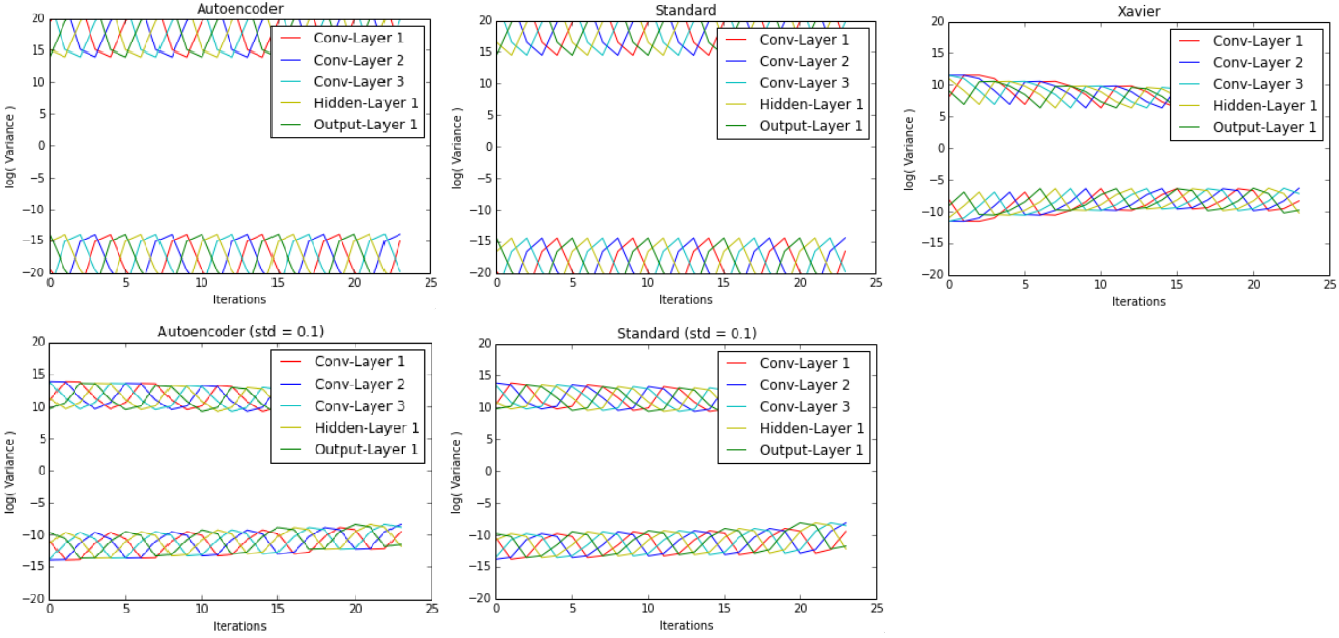
\includegraphics[width=1.0\linewidth]{images/6_xavier_initialization_cifar}
\caption[]{Log-Varianzen des Gradienten (gespiegelt) der einzelnen Schichten während der ersten Epoche des Trainings auf dem CIFAR-10A-Datensatz.}
\label{fig:6_xavier_initialization_cifar}
\end{figure}


\subsection{Gradientenabstieg}
In diesem Abschnitt werden die Adaptionen des Gradientenabstiegs untersucht, die im Rahmen dieser Arbeit von Relevanz sind. Zu diesen zählen SGD, Nesterov Momentum, RMSprop, AdaDelta und Equilibrium SGD. Da RMSprop den Equilibrium SGD sehr gut approximiert, bleibt letzterer im Folgenden unberücksichtigt. Im letzten Abschnitt konnte festgestellt werden, dass die Xavier-Initialisierung für beide Probleme eine geeignete Initialisierungsmethode darstellt. Die Experimente in diesem Teil werden deshalb mit dieser Methode initialisiert. Außerdem führt die Vorverarbeitung des CIFAR-10B-Datensatz zu einer konstanten, wenn auch kleinen, Verbesserung der Fehlerraten. Im folgenden wird deshalb lediglich der MNIST und CIFAR-10B-Datensatz betrachtet. Folgende Hyperparameter sind für alle Methoden gleich:

\begin{itemize}
\item 90 \% Trainings- und 10 \% Validierungsdaten
\item Lernrate $\eta = 0.01$
\item \textit{Early Stopping Patience} von fünf Epochen mit reduzierten Trainingsdaten und eine Epoche beim Training mit den kombinierten Trainingsdaten
\item Validierung des Modells nach jeweils 1000 Gradientenupdates (\textit{Mini-Batch}-Iterationen)
\end{itemize}

Im Rahmen der folgenden Experimente ist kein Absenken der Lernrate über das Training vorgesehen. Lediglich beim standardmäßigen SGD wird die Lernrate während des abschließenden Trainings mit kombinierten Daten auf $\eta = 0.001$ gesenkt, da diese Methode selbst keine Möglichkeit zur Veränderung der Lernrate besitzt. Neben dem \textit{Early-Stopping} werden keine weiteren Methoden zu Regularisierung verwendet. Die Tabelle \ref{tab:6_gradientdescent} zeigt eine Übersicht der jeweils erreichten Fehlerraten auf den Validierungs- und Testdaten.


\begin{table}
\centering
\begin{tabular}{c|c|c}
 	 			&   MNIST							& CIFAR-10B						 		\\ 
\hline SGD		&  0.40/0.82/0.93 \% (21 Ep.)	&	18.87/30.29/33.31 \% (27 Ep.)		\\
\hline Nesterov &  0.06/0.12/0.69 \% (11 Ep.)	&	17.77/28.94/34.01 \% (34 Ep.)				\\
\hline RMSprop  &  0.22/0.48/0.89 \% (10 Ep.)	&	29.03/37.74/41.92 \% (29 Ep.)				\\
\hline AdaDelta &  0.02/0.18/0.61 \% (12 Ep.)	&	20.86/21.99/36.65 \% (12 Ep.)				\\

%AdaDelta CIFAR 36.65
\end{tabular} 
\caption{Fehler auf den Trainings-/Validierungs-/Testdaten nach dem gesamten Training mit verschiedenen Methoden zum Gradientenabstieg}
\label{tab:6_gradientdescent}
\end{table}

In Abbildung \ref{fig:6_filters_mnist} sind Beispiele der Filter der ersten Schicht des \textit{LeNet 5+} nach dem Training mit dem MNIST-Datensatz dargestellt. Die Abbildung \ref{fig:6_filters_cifar} zeigt beispielhafte Filter der ersten Schicht des \textit{Net-7} nach dem Training mit den CIFAR-10B-Daten in Graustufen.

\begin{figure}
\centering
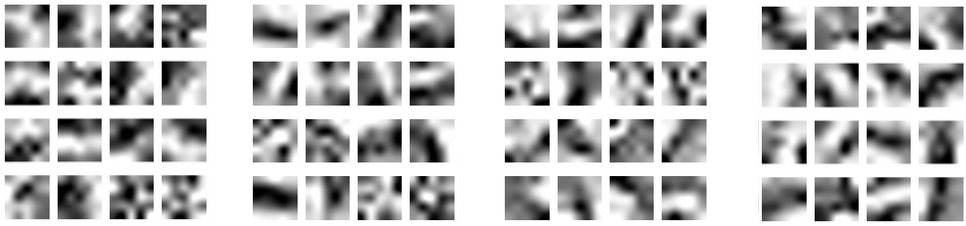
\includegraphics[width=0.7\linewidth]{images/6_filters_mnist}
\caption[]{Beispielhafte Filter der ersten Schicht des \textit{LeNet 5+}: SGD (links), Nesterov (mitte-links), RMSprop (mitte-rechts) und AdaDelta-Methode (rechts)}
\label{fig:6_filters_mnist}
\end{figure}


\begin{figure}
\centering
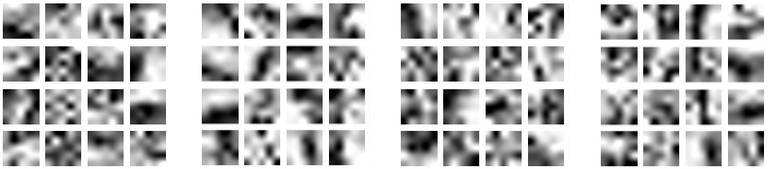
\includegraphics[width=0.7\linewidth]{images/6_filters_cifar}
\caption[]{Beispielhafte Filter der ersten Schicht des \textit{Net-7}: SGD (links), Nesterov (mitte-links), RMSprop (mitte-rechts) und AdaDelta-Methode (rechts)}
\label{fig:6_filters_cifar}
\end{figure}


\subsubsection{SGD}
Das Training auf den MNIST-Daten mit SGD dauert mit 21 Epochen im Vergleich zu den anderen Methoden sehr lange. Auch sind die erreichten Fehlerraten im Vergleich die schlechtesten. Die Abbildung \ref{fig:6_training_mnist} zeigt den Verlauf der Fehlerraten über das gesamte Training. 
Das Training mit den CIFAR-10B-Daten gestaltet sich schwieriger und dauert mit SGD 27 Epochen. Die SGD Methode erzielt im Rahmen dieser Experimente das zweitbeste Ergebnis. Allerdings ist dieses Ergebnis mit einer Fehlerrate von 33.31 \% relativ schlecht und das Training mit SGD insgesamt sehr langsam. Die Abbildung \ref{fig:6_training_cifar} zeigt den Verlauf der Fehlerraten über das gesamte Training.

\begin{figure}
\centering
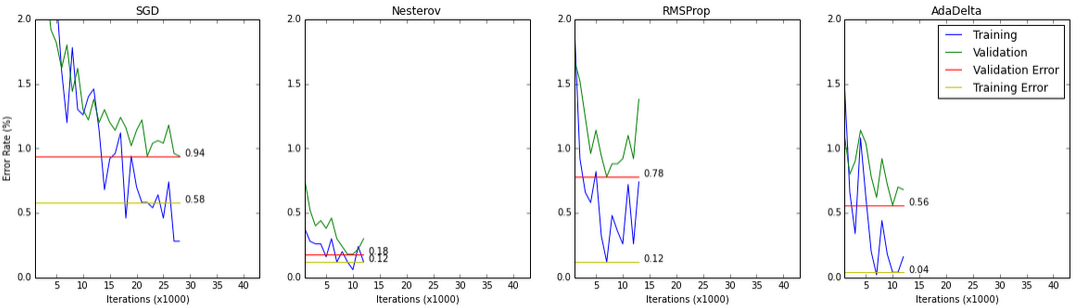
\includegraphics[width=1.0\linewidth]{images/6_training_mnist_2}
\caption[]{Trainings- und Validierungsfehler während des Trainings auf dem reduzierten MNIST-Datensatz mittels SGD-, Nesterov-, RMSprop und AdaDelta-Methode}
\label{fig:6_training_mnist}
\end{figure}


\subsubsection{Nesterov-Momentum}
Für das Training mittels Nesterov-Momentum wird als Hyperparameter für den Momentum-Term exemplarisch $\mu = 0.95$ gewählt \cite[vgl.][]{Sutskever2013}.
Das Training auf den MNIST-Daten ist deutlich beschleunigt und endet bereits nach 11 Epochen. Daneben weist es mit einem Testfehler von 0.69 \% die zweitbeste Fehlerrate auf.  
Beim Training mit den CIFAR-10B-Daten fällt auf, dass der Validierungsfehler kleiner ist als beim Training mit SGD, der Testfehler jedoch etwas höher. Das Training dauert mit 34 Epochen in Relation zu den anderen Methoden am längsten. Die Lernkurve ähnelt beim Training mit CIFAR-10B sehr jener des SGD, weist allerdings gegen Ende einen flacheren Verlauf auf und ist insgesamt weniger volatil.


\subsubsection{RMSprop}
Für das Training mit RMSprop werden folgende Werte exemplarisch als Hyperparameter gewählt \cite[vgl.][]{Dauphin2015}:
\begin{itemize}
\item $\rho = 0.90$
\item $\mu =10^{-2}$
\end{itemize}
Das Training mit RMSprop erreicht auf den MNIST-Daten nach 10 Epochen bessere Fehlerraten als der SGD, allerdings nicht so gute Ergebnisse wie die Methoden Nesterov-Momentum und AdaDelta.
Beim Training mit CIFAR-10B-Daten erzielt die RMSprop-Methode nach 29 Epochen die schlechtesten Ergebnisse im Rahmen dieser Experimente. Insgesamt weisen die Lernkurven im Vergleich zum Training mit Nesterov-Momentum einen volatileren Verlauf auf. Beim Training mit den MNIST-Daten fällt auf, dass die Fehlerraten nach dem Minimum sich sehr schnell verschlechtern.

\begin{figure}
\centering
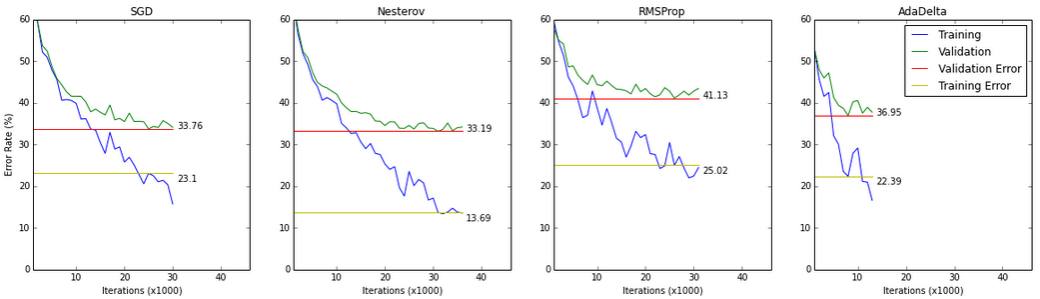
\includegraphics[width=1.0\linewidth]{images/6_training_cifar_2}
\caption[]{Trainings- und Validierungsfehler während des Trainings auf dem reduzierten CIFAR-10B-Datensatz mittels SGD-, Nesterov-, RMSprop und AdaDelta-Methode}
\label{fig:6_training_cifar}
\end{figure}

\subsubsection{AdaDelta}
Für das Training mit AdaDelta werden folgende Werte exemplarisch als Hyperparameter gewählt \cite[vgl.][]{Zeiler2012}:
\begin{itemize}
\item $\rho = 0.95$
\item $\mu = 10^{-6}$
\end{itemize}
Das Training mit AdaDelta erreicht auf den MNIST-Daten bereits nach 12 Epochen einen Testfehler von 0.61 \%. Damit erzielt die AdaDelta-Methode im Rahmen dieser Experimente die besten Ergebnisse. Ähnlich verhält es sich bei Durchführung des Experiments auf Basis der CIFAR-10B-Daten. Hier erreicht das Training mit der AdaDelta-Methode bereits nach 12 Epochen den besten Validierungsfehler und einen Testfehler im oberen Bereich. Auffällig ist, dass der Validierungsfehler beim Training mit den kombinierten Trainingsdaten sehr schnell fällt und sich damit das Modell rasch an die neuen Daten anpasst. Letztendlich handelt es sich hierbei jedoch um \textit{Overfitting}. Insgesamt weist das Training mit AdaDelta die höchste Volatilität in den Fehlerraten auf.


\subsection{Regularisierung}
Im letzten Abschnitt konnte festgestellt werden, dass der Validierungsfehler deutlich unter dem Testfehler liegt. Während das \textit{LeNet 5+} dennoch sehr gute Ergebnisse erzielt, zeigt das \textit{Net-7} bereits früh im Training eine Stagnation der Validierungsfehler. Dieses als \textit{Overfitting} bekannte Phänomen gilt es zu vermeiden. Begründen lässt sich dies damit, da ein solches Modell mit großer Sicherheit zu einem schlechteren Ergebnis auf unbekannten Daten führt, als ein regularisiertes Vergleichsmodell. In diesem Abschnitt gilt es daher entsprechende Techniken zur Regularisierung zu untersuchen.

Als Basis dient das \textit{Net-7} sowie der CIFAR-10B-Datensatz. Für den Gradientenabstieg wird die AdaDelta-Methode mit den Hyperparametern aus den vorhergegangenen Experimenten eingesetzt, da diese Methode gute Ergebnisse mit kurzer Trainingszeit erzielt. Als Referenzergebnis dienen 21.99/36.65 \% Fehlerrate auf den Validierungs-/Testdaten.
Auf die L1-Regularisierung wird im Folgenden verzichtet, da die erwünschte \textit{Sparsity} der Aktivierungen bereits durch die Verwendung von ReLu-Aktivierungsfunktionen erzielt wird (siehe. Kapitel \ref{ch:l1_l2}).
In Tabelle \ref{tab:6_regularisierung} sind die Ergebnisse der Experimente sortiert nach Testfehler aufgeführt.

\begin{table}
\centering
\begin{tabular}{c|c}
													&	 CIFAR-10B						\\ 
\hline MLP/1-Conv 0.3 \% + Max/L2 + Padd.		& 	27.61/27.06/28.41 \%	 	(21 Ep.)	\\
\hline MLP 0.3 \% + Max + Padd.				& 	16.68/21.51/29.69 \%	 	(36 Ep.)	\\
\hline MLP/1-Conv 0.3 \%  + Max + Padd.		& 	22.48/25.55/29.97 \%	 	(32 Ep.)	\\
\hline Dropout MLP 0.3 \%							& 	20.51/27.15/33.13 \% 		(20 Ep.)	\\
\hline Max-Norm-Regularisierung						& 	21.64/22.82/35.07 \% 		(18 Ep.)	\\
\hline L2-Regularisierung							& 	22.43/27.97/35.21 \% 		(21 Ep.)	\\
\hline Dropout MLP/1-Conv 0.3 \% + Max				& 	27.63/33.87/35.24 \% 		(44 Ep.)	\\
\hline Dropout MLP 0.5 \% + Max						& 	25.40/29.96/35.89 \% 		(20 Ep.)	\\
\hline Net-7 ohne Regularisierung					& 	20.86/21.99/36.65 \%		(12 Ep.)	\\
\hline Dropout MLP/1-Conv 0.5 \% + Max				& 	50.97/51.02/51.81 \% 		(27 Ep.)	\\
\end{tabular} 
\caption{Fehler auf den Trainings-/Validierungs-/Testdaten nach dem gesamten Training mit verschiedenen Methoden zur Regularisierung sortiert nach Testfehler}
\label{tab:6_regularisierung}
\end{table}


\subsubsection{L2-Regularisierung}
In diesem Experiment wird dem Modell die L2-Regularisierung hinzugefügt. Die Regularisierung wird dabei exemplarisch mit Parameter $\alpha = 0.0005$ in die Zielfunktion mit aufgenommen \cite[vgl.][]{Krizhevsky2012}.
Wird das Training wiederholt, so zeigt diese Art der Regularisierung den gewünschten Effekt. Die Tabelle \ref{tab:6_regularisierung} lässt einen erhöhten Validierungsfehler von 27.97 \% und einen etwas verbesserten Testfehler von 35.21 \% erkennen. Betrachtet man die Lernkurven in Abbildung \ref{fig:6_overfit_max_l2} zeigt das Training mit L2-Regularisierung allerdings ein sehr ähnliches Verhalten wie ohne Regularisierung und weist gerade in der Mitte des Trainings starkes \textit{Overfitting} auf. Insgesamt verlängert sich die Trainingszeit um 9 Epochen.

\begin{figure}
\centering
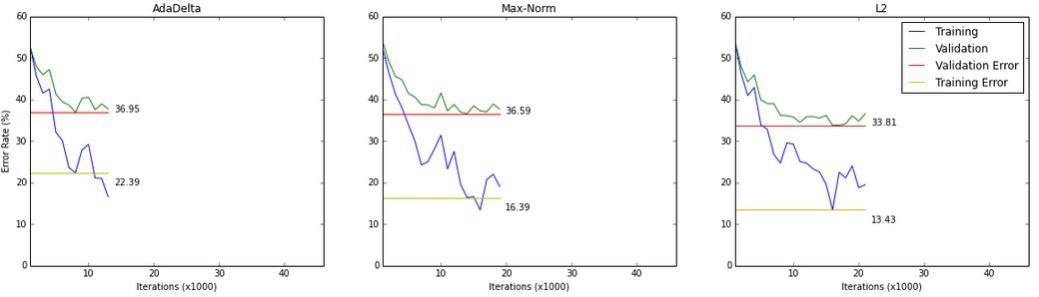
\includegraphics[width=0.8\linewidth]{images/6_overfit_max_l2_2}
\caption[]{Trainings- und Validierungsfehler während des Trainings auf dem reduzierten CIFAR-10B-Datensatz mittels AdaDelta-Methode, Max-Norm- und L2-Regularisierung}
\label{fig:6_overfit_max_l2}
\end{figure}


\subsubsection{Max-Norm-Regularisierung}
Im zweiten Experiment wird eine maximale Norm für die Gewichte festgelegt. Diese beträgt exemplarisch $ ||w||_2 <= 3  $ \cite[vgl.][]{Srivastava2014}.
Diese Art der Regularisierung hat weniger Einfluss auf das Training als die L2-Regularisierung. Dennoch wird der Validierungsfehler bei gleichzeitiger Verbesserung des Testfehlers um 1.58 \% etwas verschlechtert. Darüber hinaus ist der Testfehler in etwa gleich groß wie jener der L2-Regularisierung. Das Training mit Max-Norm-Regularisierung verhindert zu Beginn des Trainings eine Überanpassung, wie Abbildung \ref{fig:6_overfit_max_l2} zeigt. Das Training wird durch dies Regularisierung um 6 Epochen verlängert und \textit{Overfitting} tritt weiterhin sehr stark im Verlauf des Trainings auf.

\subsubsection{Dropout}
Die dritte betrachtete Methode zur Regularisierung ist das Dropout-Training. In diesen Experimenten werden zwei unterschiedliche Konfigurationen untersucht. Zuerst wird Dropout nur im Hidden-Layer des MLP angewandt. Anschließend wird die Dropout-Methode sowohl im Hidden-Layer des MLP als auch im letzten Convolution-Layer angewandt.
Als Dropout-Raten werden exemplarisch 0.3 \% und 0.5 \% untersucht (vgl. \cite{Srivastava2014}).
Im ersten Experiment wird Dropout nur im MLP verwendet. Bei beiden Dropout-Raten ist die Auswirkung auf das Training deutlich zu erkennen und der Unterschied zwischen Validierungs- und Testfehler fällt kleiner aus. Das bessere Ergebnis erreicht die Dropout-Rate von 0.3 \%, wodurch der Validierungsfehler auf 27.15 \% verschlechtert und der Testfehler gleichzeitig auf 33.13 \% verbessert wird. Ein Dropout von 0.5 \% führt hingegen zu einer Verschlechterung des Testfehler. Betrachtet man die Lernkurven in Abbildung \ref{fig:6_overfit_dropout} fällt auf, dass die Netze nach wie vor großes \textit{Overfitting} aufweisen.
Anders verhält es sich bei der zusätzlichen Anwendung von Dropout im letzten Convolution-Layer. Das Modell wird hierbei stärker regularisiert, was zu einer weiteren Verringerung des Abstandes zwischen den Fehlerraten führt. Allerdings verlängert sich die Trainingszeit deutlich. Hierbei führt eine Dropout-Rate von 0.3 \% zu einem etwas besseren Ergebnis als das Training ohne Regularisierung. Eine Dropout-Rate von 0.5 \% hingegen beschränkt das Modell sehr stark und das Ergebnis verschlechtert sich. Die Lernkurven weisen bei Dropout in mehreren Schichten jedoch deutlich weniger \textit{Overfitting} auf.

\begin{figure}
\centering
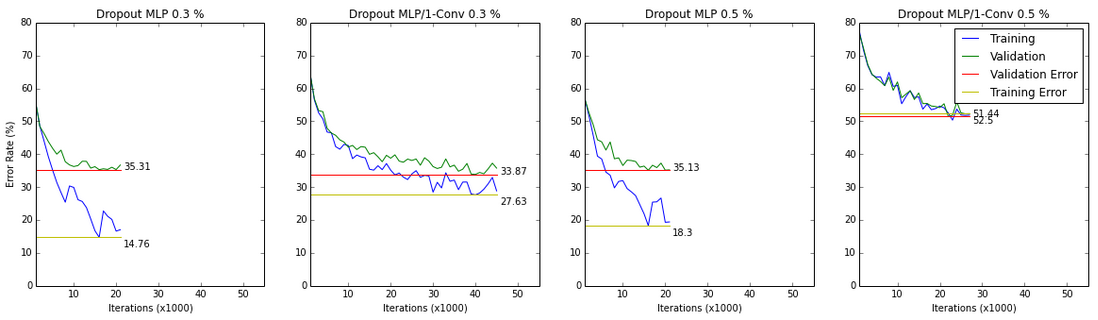
\includegraphics[width=1.0\linewidth]{images/6_overfit_dropout_2}
\caption[]{Trainings- und Validierungsfehler während des Trainings auf dem reduzierten CIFAR-10B-Datensatz mittels Dropout}
\label{fig:6_overfit_dropout}
\end{figure}

\subsubsection{Padding}
Die letzten Experimente zeigen, dass sowohl die L2-Regularisierung als auch das Dropout-Training zu einem kleinerem Abstand zwischen dem Validierungs- und Testfehler führen können. Die folgenden Experimente sollen die Auswirkung von Padding in den Convolution-Layern zeigen. Zusätzlich zum Padding wird die Dropout-Regularisierung mit einer Rate von 0.3 \% sowie die Max-Norm- und L2-Regularisierung aus den letzten Experimenten verwendet.
Durch Padding wird die Größe der Eingabe nur in den Pooling-Layern verringert. Damit erhöht sich die Dimension der Ausgabe des letzten Convolution-Layers von 64 auf 1024, was zu deutlich mehr trainierbaren Gewichten im MLP führt.\footnote{Hier wird in den Convolution-Layern aus Gründen der Implementierung Ausgabe-Padding eingesetzt und die CIFAR-10B-Eingaben werden entsprechend vor dem Training auf die Größe $36 \times 36$ vergrößert. Außerdem entfällt somit das Padding der Ausgabe des letzten Convolution-Layers.}

Wie das erste Experiment zeigt, steigt hierdurch die Kapazität des Modells deutlich und der Testfehler verbessert sich bei Dropout im MLP auf 29.69 \%. Im Vergleich zum Modell ohne Padding tritt am Ende außerdem ein größeres \textit{Overfitting} auf, durch Nutzung von Dropout allerdings weniger als im Modell ohne Regularisierung. Insgesamt zeigen die Lernkurven in Abbildung \ref{fig:6_overfit_padding} einen ähnlichen Verlauf wie jene des Trainings ohne Padding. Der größere Hidden-Layer im MLP wird oftmals durch die Max-Norm-Regularisierung regularisiert, was zu einem volatileren Verlauf im Trainingsfehler führt. 
Wird das Dropout-Training zusätzlich im letzten Convolution-Layer angewandt, wird das \textit{Overfitting} deutlich verringert, allerdings verschlechtert sich der Testfehler etwas.
Auffällig ist, dass das Modell hierbei weniger regularisiert wird als ohne Padding. Wird zusätzlich die L2-Regularisierung aktiviert, wird das \textit{Overfitting}, bei gleichzeitiger Verbesserung des Testfehlers und verkürzter Trainingszeit, deutlich reduziert.

\begin{figure}
\centering
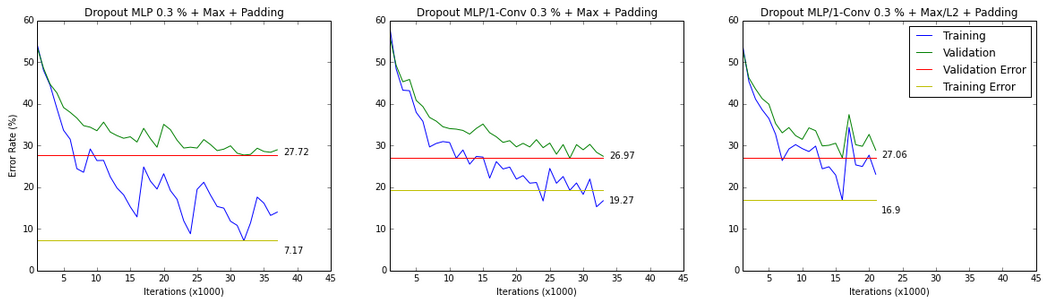
\includegraphics[width=0.8\linewidth]{images/6_overfit_padding_2}
\caption[]{Trainings- und Validierungsfehler während des Trainings auf dem reduzierten CIFAR-10B-Datensatz mittels Dropout und Padding}
\label{fig:6_overfit_padding}
\end{figure}


\subsubsection{Modellkapazität}
Durch die Kombination von Padding, Dropout und Max-Norm- sowie L2-Regularisierung kann ein gewünschtes Ergebnis mit guter Generalisierung erzielt werden. Die folgenden Experimente sollen die Auswirkung der Modellkapazität und damit die Größe des Modells aufzeigen. Dazu werden zwei neue Modelle eingeführt, wobei das ein im Vergleich zum \textit{Net-7} eine Vergrößerung darstellt, das andere eine Verkleinerung. Beide neuen Netze verwenden ebenfalls Ausgabe-Padding.

\begin{table}
\centering
\begin{tabular}{c|c}
															& CIFAR-10B						 	\\ 
\hline \textit{Net-8} MLP/1-Conv 0.3 \% + L2/Max	& 	21.92/23.32/27.50 \%	 	(25 Ep.)	\\ %27.94
\hline \textit{Net-8} MLP/1-Conv 0.3 \% + Max		& 	16.15/21.20/27.55 \%	 	(27 Ep.)	\\
\hline \textit{Net-8} MLP 0.3 \% + Max				& 	13.30/13.26/27.84 \%	 	(25 Ep.)	\\
\hline \textit{Net-7-Small}	+ L2							& 	30.33/31.02/35.35 \% 		(37 Ep.)	\\
\hline Net-7 ohne Regularisierung							& 	20.86/21.99/36.65 \%		(12 Ep.)	\\
\hline \textit{Net-7-Small}	+ Max							& 	29.85/31.86/36.69 \% 		(20 Ep.)	\\
\end{tabular} 
\caption{Fehler auf den Trainings-/Validierungs-/Testdaten nach dem gesamten Training mit \textit{Net-7-Small} und \textit{Net-8} unter Verwendung verschiedener Methoden zur Regularisierung sortiert nach Testfehler}
\label{tab:6_regularisierung2}
\end{table}

Die Ergebnisse der einzelnen Experimente werden in Tabelle \ref{tab:6_regularisierung2} sortiert nach Testfehler aufgeführt. \\

\textit{Net-7-Small} \\
Das erste Netz, welches genutzt werden soll, besitzt keinen Hidden-Layer und die Anzahl der \textit{Feature-Maps} ist auf 20 reduziert. Es orientiert sich am Modell von \cite{Kaparthy2014}. Insgesamt besitzt dieses Netz lediglich 24.700 Gewichte, wobei die Architektur durch Padding einen weiteren Pooling-Layer nach dem letzten Convolution-Layer erlaubt.
Das Modell wird mit 20-20-20/10 abgekürzt und umfasst im Detail die folgenden sieben Schichten:
\begin{enumerate}
\setlength{\itemsep}{0pt}
\item Convolution-Layer: 20 \textit{Feature-Maps} mit $5 \times 5$ Filtermasken
\item Pooling-Layer:	$2 \times 2$ Filtermasken
\item Convolution-Layer: 20 \textit{Feature-Maps} mit $5 \times 5$ Filtermasken
\item Pooling-Layer:	$2 \times 2$ Filtermasken
\item Convolution-Layer: 20 \textit{Feature-Maps} mit $5 \times 5$ Filtermasken
\item Pooling-Layer:	$2 \times 2$ Filtermasken
\item Output-Layer: 10 Neuronen mit Cross-Entropy Fehlermaß
\end{enumerate}



\begin{figure}
\centering
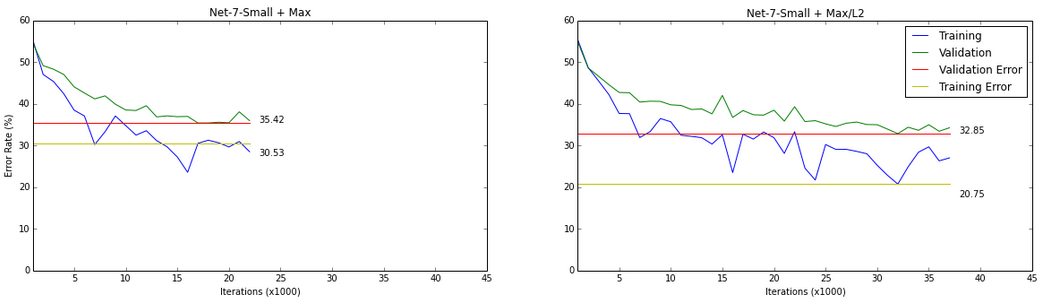
\includegraphics[width=0.7\linewidth]{images/6_overfit_small_2}
\caption[]{Trainings- und Validierungsfehler während des Trainings auf dem reduzierten CIFAR-10B-Datensatz mittels \textit{Net-7-Small} sowie Max-Norm- und L2-Regularisierung}
\label{fig:6_overfit_small}
\end{figure}

Die Ergebnisse in Tabelle \ref{tab:6_regularisierung2} zeigen, dass das verkleinerte \textit{Net-7-Small} nahezu dasselbe Ergebnis wie das \textit{Net-7} erreicht. Gleichzeitig erreicht es eine bessere Generalisierung und benötigt eine kürzere Trainingszeit. Wird jedoch zusätzlich die L2-Regularisierung angewandt, verlängert sich die Trainingszeit hinsichtlich der durchlaufenen Epochen immens. Die Abbildung \ref{fig:6_overfit_small} zeigt auf, dass die Lernkurve hierbei einen flacheren Verlauf aufweist. Insgesamt verringert die Verkleinerung des Netzes das \textit{Overfitting} deutlich und führt bei zusätzlicher L2-Regularisierung zu einem besseren Testfehler.\\


\textit{Net-8} \\
Beim zweiten Netz werden die Anzahl der \textit{Feature-Maps} sowie die Anzahl der Neuronen im Hidden-Layer erhöht. Es stellt eine etwas kleinere Variante des Modells von \cite{Masci2011} dar. Insgesamt besitzt dieses Netz 510.100 Gewichte. Durch Padding erlaubt die Architektur, wie das \textit{Net-7-Small}, einen weiteren Pooling-Layer nach dem letzten Convolution-Layer, wodurch sich die Anzahl der Schichten auf acht erhöht.
Das Modell wird mit 100-100-100/100-10 abgekürzt und umfasst im Detail die folgenden acht Schichten:
\begin{enumerate}
\setlength{\itemsep}{0pt}
\item Convolution-Layer: 100 \textit{Feature-Maps} mit $5 \times 5$ Filtermasken
\item Pooling-Layer:	$2 \times 2$ Filtermasken
\item Convolution-Layer: 100 \textit{Feature-Maps} mit $5 \times 5$ Filtermasken
\item Pooling-Layer:	$2 \times 2$ Filtermasken
\item Convolution-Layer: 100 \textit{Feature-Maps} mit $5 \times 5$ Filtermasken
\item Pooling-Layer:	$2 \times 2$ Filtermasken
\item Hidden-Layer: 100 Neuronen
\item Output-Layer: 10 Neuronen mit Cross-Entropy Fehlermaß
\end{enumerate}


Mit dem vergrößerten Netz steigt die Kapazität des Netzes im Vergleich zum \textit{Net-7} mit Padding nochmals, was zu den besseren Fehlerraten führt, die in Tabelle \ref{tab:6_regularisierung2} aufgeführt sind. Das Netz weist am Ende ebenfalls ein großes \textit{Overfitting} auf und die Lernkurven in Abbildung \ref{fig:6_overfit_big} weisen einen ähnlichen Verlauf wie die Kurven im \textit{Net-7} auf. Wird das Netz mit L2-Regularisierung trainiert, verbessert sich die Generalisierung und das Netz erreicht den besten Testfehler im Rahmen dieser Experimente. 

\begin{figure}
\centering
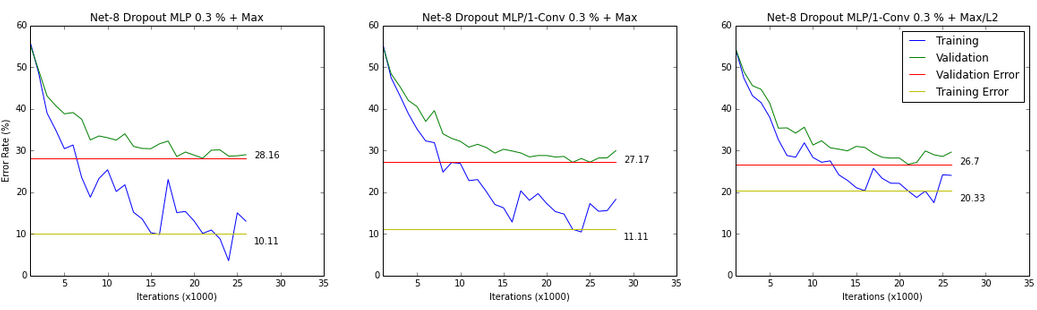
\includegraphics[width=0.8\linewidth]{images/6_overfit_big_2}
\caption[]{Trainings- und Validierungsfehler während des Trainings auf dem reduzierten CIFAR-10B-Datensatz mittels \textit{Net-8} mit Max-Norm- und L2-Regularisierung sowie Dropout}
\label{fig:6_overfit_big}
\end{figure}

	
\section{Visualisierung}
Neben der Darstellung der Filtermasken existieren zur Visualisierung weitere nützliche Methoden.
Im folgenden Teil soll die Anwendung zweier zentraler Techniken zur Visualisierung von CNNs gezeigt werden. Einerseits die sogenannte Neuronen-Visualisierung zur Rekonstruktion der Aktivierung eines beliebigen Neurons, andererseits die t-SNE zur Dimensionsreduktion. Darüber hinaus werden mittels des Convolutional Autoencoders die Aktivierungen im CNN untersucht.
	

\subsection{Neuronen-Visualisierung}
Mit der Neuronen-Visualisierungen können einzelne aktivierte \textit{Feature-Maps} in den Eingaberaum zurück propagiert werden. Bis auf wenige Anpassungen, funktioniert diese analog zum \textit{Backward Pass} des Backpropagation-Algorithmus.


\begin{figure}
\centering
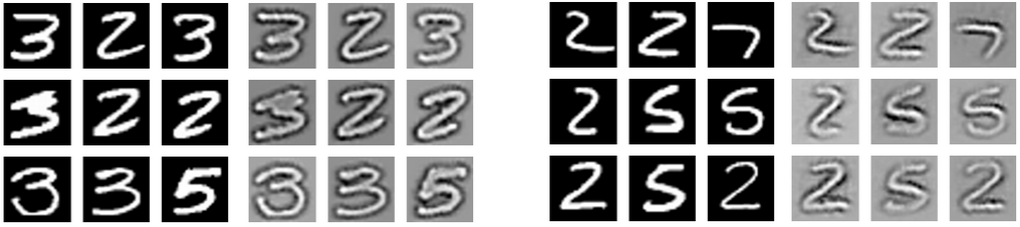
\includegraphics[width=1.0\linewidth]{images/6_visualize_mnist}
\caption[]{Visualisierung der neun stärksten Aktivierungen im \textit{LeNet 5+} mit der Methode von \cite{Zeiler2014} auf den gesamten Testdaten:  Erste \textit{Feature-Map} in der zweiten Schicht (links) und erste \textit{Feature-Map} in der vierten Schicht (rechts)}
\label{fig:6_vis_mnist}
\end{figure}


Im folgenden soll die Methode von \cite{Zeiler2014} angewandt werden, um beispielhafte Neuronen zu visualisieren. Abbildung \ref{fig:6_vis_mnist} zeigt je eine \textit{Feature-Map} der zweiten sowie der vierten Schicht eines mit MNIST-Daten trainierten \textit{LeNet 5+}. Die \textit{Feature-Map} der ersten Schicht fungiert eindeutig als Kantendetektor, was auch bei der Betrachtung der Filtermasken in Abbildung \ref{fig:6_filters_mnist} plausibel erscheint. Interessanter erscheint die \textit{Feature-Map} der vierten Schicht. Diese scheint gerade Kanten besonders zu detektieren, was bei den Ziffern fünf und sieben besonders auffällt.



Wird dieselbe Methode auf ein mit CIFAR-10B-Daten trainiertes \textit{Net-8} angewandt, ergeben sich die Rekonstruktionen in Abbildung \ref{fig:6_vis_cifar}, wobei jeweils der V-Kanal dargestellt ist. Hier werden jeweils zwei \textit{Feature-Maps} in der zweiten und vierten Schicht gezeigt. Wie auch im \textit{LeNet 5+} fungieren die Filtermasken der zweiten Schicht als Kantendetektoren. Darüber hinaus detektieren sie bei Farbbildern die Tönung des Bildes. Die obere \textit{Feature-Map} der vierten Schicht hingegen scheint, bis auf zwei Ausnahmen, Schiffe zu detektieren. Betrachtet man die Rekonstruktionen, ist erkennbar, dass besonders die länglichem Kanten erkannt werden. Außerdem weist die Rekonstruktion der Aktivierung des oberen Autos starke Ähnlichkeit zu einem Boot auf. Die zweite \textit{Feature-Map} detektiert augenscheinlich längliche Objekte. Diese lassen sich alleine mit dieser \textit{Feature-Map} nicht einzelnen Klassen zuordnen. Dennoch weist diese eine gewissen Relevanz auf, da sowohl drei sehr ähnliche Tarnkappen-Flugzeuge und drei sitzende Katzen detektiert werden. 

\begin{figure}
\centering
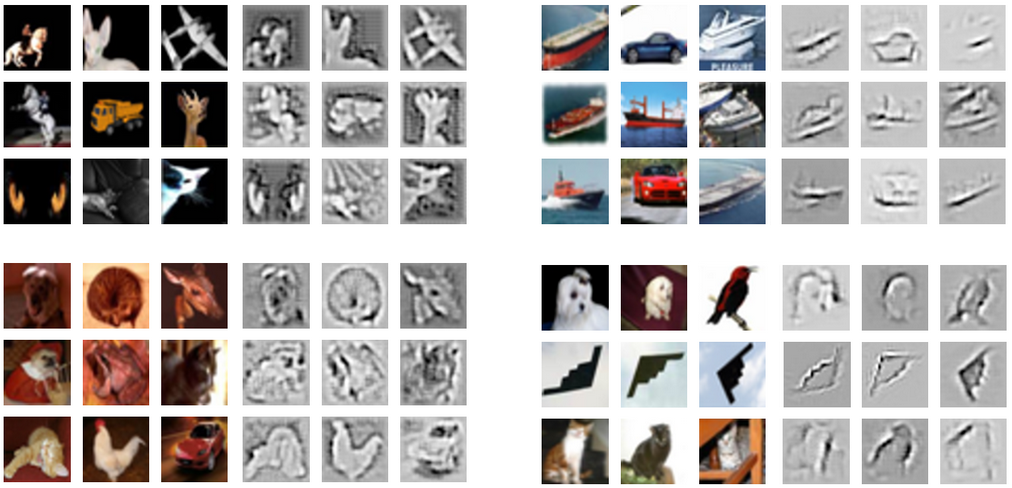
\includegraphics[width=1.0\linewidth]{images/6_visualize_cifar}
\caption[]{Visualisierung der neun stärksten Aktivierungen im \textit{Net-8}  mit der Methode von \cite{Zeiler2014} auf den gesamten Testdaten: Erstes und neuntes Neuron in der zweiten Schicht (links) und erstes und neuntes Neuron in der vierten Schicht (rechts)}
\label{fig:6_vis_cifar}
\end{figure}


\subsection{t-SNE-Methode}
Die t-SNE-Methode von \cite{Laurens2008} kann wie die Hauptkomponentenanalyse (PCA) zur Dimensionsreduktion eingesetzt werden. Im Unterschied zur PCA berücksichtigt diese bei der Reduktion alle Hauptkomponenten. An dieser Stelle wird t-SNE verwendet, um die von den Convolution-Layern extrahierten Merkmale im 2D-Bildraum zu visualisieren. Die t-SNE wird im Folgenden ausgehend von den ersten 50 Hauptkomponenten 1000 Iterationen lange gerechnet.

Abbildung \ref{fig:6_tsne_mnist} zeigt zufällige 2500 originale sowie durch das CNN transformierte MNIST-Beispiele in einem Streudiagramm. Es ist deutlich erkennbar, dass die zehn Klassen nach den beiden Convolution-Layern des \textit{LeNet 5+} kompaktere Gruppen bilden. Dies ermöglicht eine bessere Trennung der Daten im nachfolgenden mit abschließender Softmax-Regression.

\begin{figure}
\centering
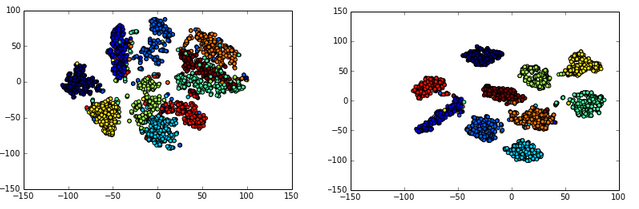
\includegraphics[width=0.9\linewidth]{images/6_tsne_mnist}
\caption[]{Visualisierung von 2500 MNIST-Beispielen mit t-SNE im Original (links) und nach der vierten Schicht des trainierten \textit{LeNet 5+} (rechts)}
\label{fig:6_tsne_mnist}
\end{figure}

Für die Visualisierung der CIFAR-10B-Daten wird eine andere Methode gewählt. An Stelle des Streudiagramms werden die einzelnen Beispiele selbst dargestellt. Die Abbildungen \ref{fig:6_tsne_cifara} und \ref{fig:6_tsne_cifarb} zeigt 1000 originale sowie durch das CNN transformierte CIFAR-10B-Beispiele. Hierbei fällt zum einen auf, dass die Originale eindeutig anhand des Hintergrunds getrennt werden, während die Farbtöne in der Variante des CNNs etwas verwaschener sind. Darüber hinaus sind in der Punktwolke mit den extrahierten Merkmalen Lücken erkennbar. Bei genauer Betrachtung kann, beispielsweise anhand des grünen Autos im Original rechts in der Mitte, die Gruppenbildung nach Inhalt, statt nach Hintergrund oder Farbtons  festgestellt werden. Das genannte grüne Auto befindet sich nach Anwendung der Convolution-Layer bei den anderen Autos links in der Mitte. Außerdem ist die rötliche Gruppe unten-rechts bei Anwendung der t-SNE mit extrahierten Merkmalen aufgelöst.


\begin{figure}[H]
\centering
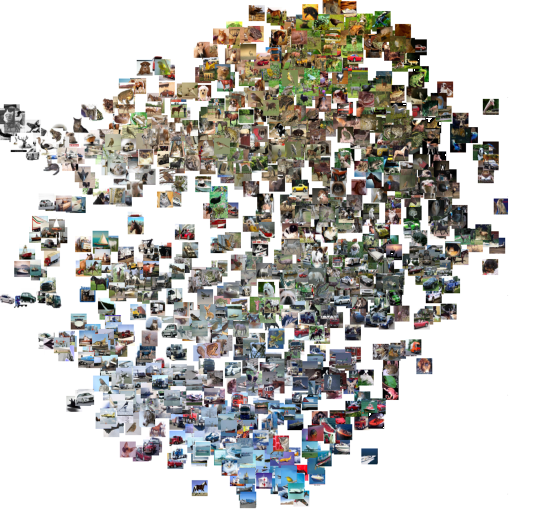
\includegraphics[width=0.8\linewidth]{images/6_cifar_tsne_combined_white_small2a}
\caption[]{Visualisierung von 1000 CIFAR-10-Beispielen mit t-SNE im Original}
\label{fig:6_tsne_cifara}
\end{figure}

\begin{figure}[H]
\centering
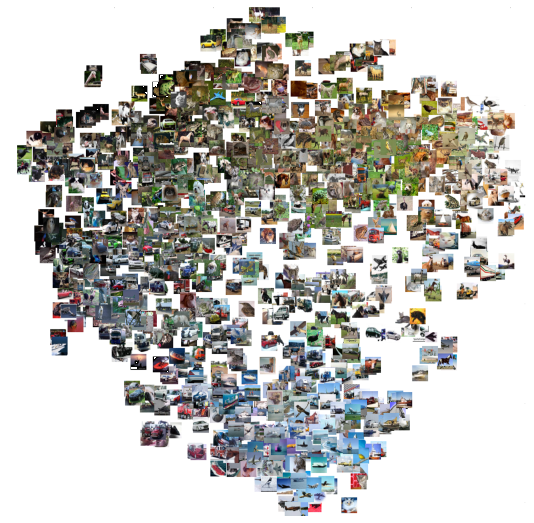
\includegraphics[width=0.8\linewidth]{images/6_cifar_tsne_combined_white_small2b}
\caption[]{Visualisierung von 1000 CIFAR-10B-Beispielen mit t-SNE nach der sechsten Schicht des trainierten \textit{Net-8}}
\label{fig:6_tsne_cifarb}
\end{figure}
		

\subsection{Autoencoder-Visualisierung}		
Der eingangs zum unüberwachten Vortraining untersuchte Convolutional Autoencoder kann ebenso zur Visualisierung verwendet werden. Dazu wird zunächst die Aktivierung für Beispieldaten in einer bestimmten Schicht berechnet. Anschließend wird diese Aktivierung anstatt des Verfahrens von \cite{Zeiler2014} mit dem Decoder des Convolutional Autoencoders in den Bildraum zurück propagiert. Die Schichten mit Max-Pooling werden zwecks Umkehrbarkeit mit Average-Pooling ausgestattet.

\begin{figure}[H]
\centering
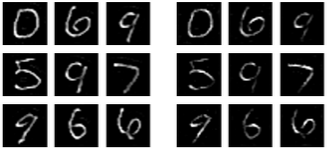
\includegraphics[width=0.4\linewidth]{images/6_visualize_mnist_autoenc}
\caption[]{Zufälligen MNIST-Beispiele im Original (links) und visualisiert mit der Autoencoder-Methode auf Basis der Aktivierungen in der vierten Schicht im \textit{LeNet 5+} (rechts)}
\label{fig:6_visualize_mnist_autoenc}
\end{figure}

Die Abbildung \ref{fig:6_visualize_mnist_autoenc} zeigt dieses Verfahren angewandt auf zufällige MNIST-Beispiele, wobei die Rekonstruktionen auffällig gut sind. Durch die ReLu-Aktivierung verschwinden außerdem negative Werte und der Hintergrund ist im Unterschied zur Methode von \cite{Zeiler2014} schwarz. Dies ist eine sehr interessante Feststellung, da die verschiedenen Filtermasken nicht mittels Autoencoder trainiert wurden. Darüber hinaus erklärt dies, warum unüberwachtes Vortraining im Deep Learning eine geeignete Methode für das Training der Filtermasken darstellt. 
	
\subsubsection{Maskierung von Merkmalen}
\begin{figure}
\centering
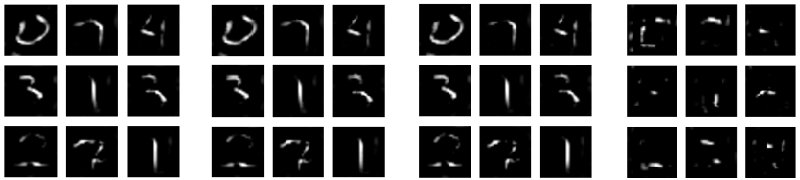
\includegraphics[width=0.8\linewidth]{images/6_visualize_mnist_autoenc2}
\caption[]{Mittels der Autoencoder-Methode visualisierte, zufällige MNIST-Beispiele mit verdeckter zehnter \textit{Feature-Map} (links), zwanzigster (mitte-links), den ersten vier (mitte-rechts) und allen ab der vierten \textit{Feature-Map} (rechts) auf Basis der Aktivierungen in der vierten Schicht im \textit{LeNet 5+}}
\label{fig:6_visualize_mnist_autoenc2}
\end{figure}

Die beschriebene Methode erlaubt ein weiteres Experimente hinsichtlich der Aktivierungen einer Schicht.
Die Abbildung \ref{fig:6_visualize_mnist_autoenc2} zeigt vier mittels Autoencoder rekonstruierte Aktivierungen. Bei den ersten Rekonstruktionen wurde die zehnte \textit{Feature-Map} der vierten Schicht verdeckt, bei den zweiten Rekonstruktionen die zwanzigste, bei den dritten die ersten vier und bei den vierten alle, außer die ersten vier. Interessanterweise sehen die ersten drei Rekonstruktionen nahezu identisch aus, während jene der vierten Abbildung kaum mehr zu erkennen sind. Dies zeigt, dass sich einzelne \textit{Feature-Maps} nicht an einzelnen Trainingsbeispielen orientieren, sondern, im Sinne der \textit{Distributed Representation}, die Kombination aus Merkmalen wichtig ist \cite[vgl.][]{Hinton1986}.

In Abbildung \ref{fig:6_cov_mnist_1_8_18} sind mehrere Kovarianzen mit spaltenweise addiertem Mittelwert dargestellt. Im ersten Bild wird die Kovarianzmatrix aller Aktivierungen der vierten Schicht mit der Ziffer 1 berechnet, im zweiten jene der Ziffer 8 und im dritten die Kombination der Ziffern 1 und 8. Insgesamt besitzt die vierte Schicht 800 Merkmale, wobei jede \textit{Feature-Map} davon 16 bündelt.	
Zunächst fällt auf, dass bei der Ziffer 1 der Mittelwert der 21. \textit{Feature-Map} die anderen dominiert. Außerdem ist die Information über mehrere Merkmale verteilt, was die erhöhten Kovarianzen innerhalb der Zeile zeigen. Analog verhält es sich bei den Aktivierungen der Ziffer 8. Darüber hinaus sind in der Kombination der Ziffern entsprechend beide Muster in den Aktivierungen erkennbar, wobei die Mittelwerte der 21. und 22. \textit{Feature-Maps} dominieren.


\begin{figure}
\centering
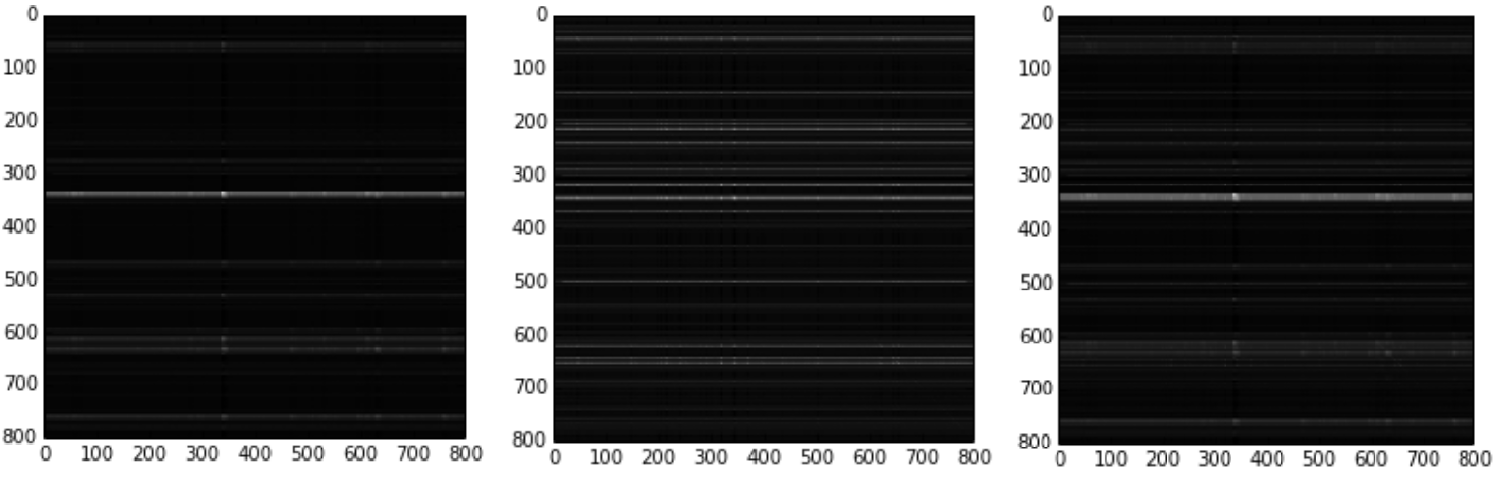
\includegraphics[width=0.6\linewidth]{images/6_cov_mnist_1_8_18}
\caption[]{Kovarianzmatrix der Aktivierungen der vierten Schicht im \textit{LeNet 5+} auf Basis aller MNIST-Beispiele mit der Ziffer 1 (links), der Ziffer 8 (mitte) und den Ziffern 1 und 8 (rechts)}
\label{fig:6_cov_mnist_1_8_18}
\end{figure}

\begin{figure}
\centering
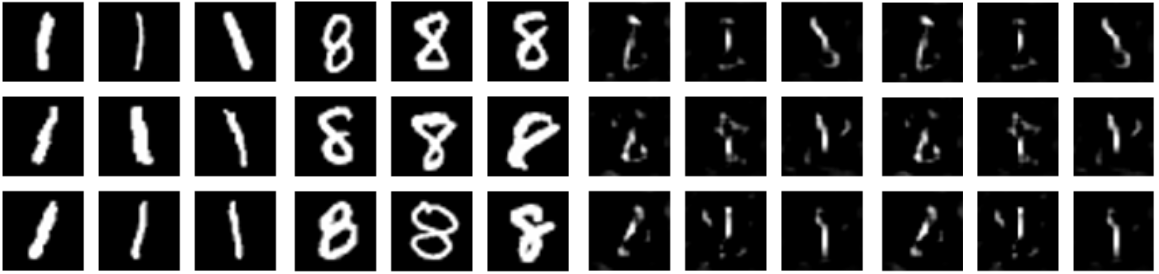
\includegraphics[width=0.6\linewidth]{images/6_visualize_mnist_autoenc_8_1}
\caption[]{Neun zufälligen MNIST-Beispielen mit der Ziffer 1 und 7 im Original (links) und visualisiert mit der Autoencoder-Methode auf Basis der gemittelten Merkmalen (mitte-rechts) und addierten Merkmalen (rechts) nach der vierten Schicht im \textit{LeNet 5+}}
\label{fig:6_visualize_mnist_autoenc_8_1}
\end{figure}


\subsubsection{Kombination von Merkmalen}

Im letzten Experiment konnte festgestellt werden, dass mehrere \textit{Feature-Maps} bei ähnlichen Eingaben korrelieren. In einem abschließenden Experiment soll die Kombination der Aktivierungen in der vierten Schicht und folglich eine Merkmalskombination visualisiert werden. Die Abbildung \ref{fig:6_visualize_mnist_autoenc_8_1} zeigt einerseits die originalen Eingaben und andererseits, auf Basis der kombinierten Merkmale der Ziffern 1 und 8, die entsprechenden Rekonstruktionen. In den Rekonstruktionen ist eindeutig erkennbar, dass die Mischung von Merkmalen zu einer entsprechenden Vermischung im Eingaberaum führt und somit entartete Kombinationen aus den Ziffern 1 und 8 entstehen. Dabei hat interessanterweise die Stärke der Aktivierung wenig Einfluss auf das Ergebnis, was der Vergleich der Rekonstruktionen mit und ohne Mittelung zeigt.

Weiterführend können auf Basis der Aktivierungen, analog zum Verfahren von \cite{Vincent2010}, auch mittels Convolutional Autoencoder synthetische \textit{Samples} erzeugt werden. Diese Methode wird allerdings in dieser Arbeit nicht näher betrachtet.




%\begin{figure}
%\centering
%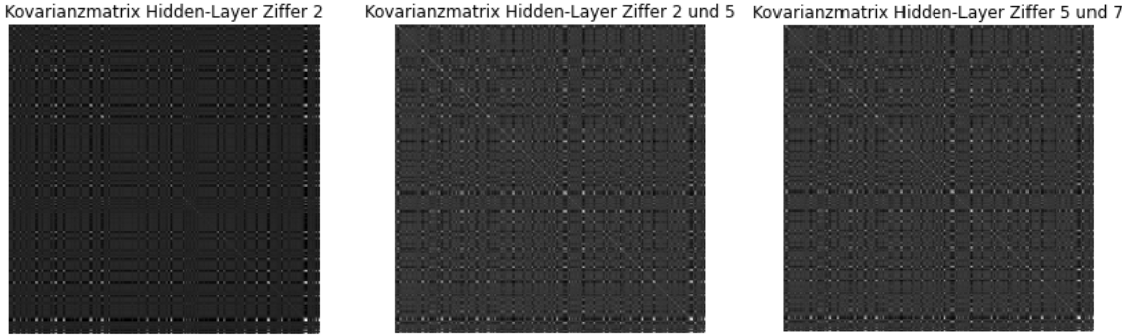
\includegraphics[width=0.6\linewidth]{images/6_cov_mnist_hidden}
%\caption[]{25 zufälligen MNIST-Beispielen im Original (links) und visualisiert mit der %Autoencoder-Methode auf Basis der Aktivierungen in der vierten Schicht im \textit{LeNet 5+} (rechts)}
%\label{fig:6_cov_mnist_hidden}
%\end{figure}


	
		
% erstmal nicht beachtet\hline Dropout ALL 0.3 \% + Max								& 	51.07/49.94 \%	 	(xx Ep.)	\\
% no Pooling \hline Dropout ALL 0.3 \% + Max-Norm + Pad/Mask 				& 	51.64/51.93 \%	 	(xx Epochen)	\\
% no Pooling \hline Dropout MLP 0.3 \% + Max-Norm + Padding					& 	19.74/31.79 \%	 	(xx Epochen)	\\
%\hline \textit{7-Net}-Small	+ L2/Max-Norm + Padding	+ Long				& 	30.36/35.46 \% 		(xx Epochen)	\\
% erstnal nicht beachtet \hline L2-Regularisierung + No MLP					& 	27.73/37.75 \% 		(xx Epochen)	\\
% erstmal nich beachtet \hline \textit{7-Net}-Big Dropout MLP 0.3 \% + Max-Norm 			& 	00.00/00.00 \%	 	(xx Epochen)	\\
%\hline \textit{7-Net}-Big Dropout MLP 0.3 \% + Max-Norm + Padding + Long	& 	00.00/00.00 \%	 	(xx Epochen)	\\		
		